\documentclass[12pt,letterpaper]{article}
\usepackage[margin=1in]{geometry}
\usepackage{mathptmx}
\usepackage{amsmath,amssymb}
\usepackage{booktabs}
\usepackage{hyperref}
\usepackage{titlesec}
\usepackage{enumitem}
\usepackage{tikz}
\usetikzlibrary{arrows.meta,positioning,shapes.geometric,calc,fit}

\hypersetup{
    colorlinks=true,
    linkcolor=black,
    urlcolor=blue,
    citecolor=black
}

\titlespacing*{\section}{0pt}{10pt}{4pt}
\titlespacing*{\subsection}{0pt}{8pt}{3pt}
\setlength{\parindent}{0pt}
\setlength{\parskip}{5pt}
\sloppy

\begin{document}

% ============================================================================
% USPTO PROVISIONAL PATENT APPLICATION HEADER
% ============================================================================
\begin{center}
    {\large \textbf{UNITED STATES PATENT AND TRADEMARK OFFICE (USPTO)\\PROVISIONAL PATENT APPLICATION UNDER 35 U.S.C.\ \S\ 111(b)}}\\[8pt]
    {\LARGE \textbf{APPARATUS, SYSTEMS, AND METHODS FOR NATIVE 16-DIMENSIONAL SEDENION SIGNAL PROCESSING, PRE-ADC ANALOG ZERO-DIVISOR INTERFERENCE CANCELLATION, SINGLE-SNAPSHOT NON-ASSOCIATIVE CURVATURE SPOOFING DETECTION, AND ZERO-DIVISOR KEYED MODULATION}}\\[10pt]
\end{center}

\begin{tabular}{@{}p{2.2in}p{4.1in}@{}}
\toprule
\textbf{Inventor / Applicant:} & Dionisio Chiuratto Agourakis \\
\textbf{Residence / Citizenship:} & S\~ao Paulo, SP, Brazil (Citizen of Brazil) \\
\textbf{Correspondence Address:} & Rua Joaquim Floriano 1125, apt 102, S\~ao Paulo, SP 04534-002, Brazil \\
\textbf{Electronic Mail / Phone:} & \texttt{dionisio.ca@gmail.com} \quad | \quad +55 11 98787-4110 \\
\textbf{Assignee / Entity Status:} & Unassigned / Micro-Entity Status (35 U.S.C.\ \S\ 123) \\
\textbf{International Priority:} & Paris Convention Priority Claimed (USPTO \& INPI Brazil) \\
\bottomrule
\end{tabular}

\section*{CROSS-REFERENCE TO RELATED DISCLOSURES (35 U.S.C.\ \S\ 102(b)(1))}
This Provisional Patent Application claims the benefit of the one-year statutory grace period under 35 U.S.C.\ \S\ 102(b)(1)(A) (United States) and Article 12 of Law No.\ 9.279/96 (Brazil INPI) with respect to the inventor's own technical disclosures: (1) Dionisio Chiuratto Agourakis, \textit{``Sedenion Algebras and PG(3,2) Incidence Structures for Non-Associative Geometric Deep Learning: Algebraic Foundations, Machine-Checked Theorems, and Dual-Track Validation,''} Zenodo DOI \texttt{10.5281/zenodo.23588274} (October 2026); and (2) Dionisio Chiuratto Agourakis, \textit{``Matrix-Inversion-Free O(1) Sedenion PG(3,2) Zero-Divisor Beamforming for Assured PNT, +80 dB GNSS Anti-Jamming, and Anti-Spoofing,''} Zenodo DOI \texttt{10.5281/zenodo.23603006} (October 2026). Both disclosures are incorporated herein by reference in their entirety.

\section*{FIELD OF THE INVENTION}
The present invention relates generally to electromagnetic array signal processing, radio-frequency (RF) interference cancellation, satellite navigation (GNSS) anti-jamming and anti-spoofing, analog-to-digital front-end protection, and low-probability-of-intercept / low-probability-of-detection (LPI/LPD) physical-layer communications. More specifically, the invention relates to physical sensor feeds, pre-ADC passive/switched analog differential crossbar networks, single-snapshot non-associative curvature detectors, and digital/mixed-signal processors operating natively in the 16-dimensional Cayley--Dickson sedenion algebra $\mathbb{S} \cong \mathbb{O} \oplus \mathbb{O}e_8$ and the finite projective geometry $\mathrm{PG}(3,2)$.

\section*{BACKGROUND OF THE INVENTION}
All conventional multi-antenna digital signal processing (DSP), phased-array radar, and Controlled Reception Pattern Antenna (CRPA) receivers formulate received wavefields as vectors in an $N$-dimensional complex Hilbert space $\mathbb{C}^N$ governed by associative, commutative complex scalar multiplication. While foundational, the $\mathbb{C}^N$ linear-algebraic paradigm suffers from four fundamental physical and computational limitations in contested electromagnetic environments:

\textbf{1. Pre-Beamformer ADC Saturation and Clipping:} In conventional Digital Beamforming (DBF), raw RF/IF signals from $N$ antenna elements are digitized by Analog-to-Digital Converters (ADCs) prior to spatial null-steering. Under high-power Electronic Attack (EA) where the Jammer-to-Signal Ratio ($\mathrm{JSR}$) reaches $+60\text{ dB}$ to $+80\text{ dB}$, the jammer waveform exceeds the full-scale dynamic range of 12-bit to 16-bit ADCs, causing severe non-linear clipping and intermodulation distortion that destroys the buried desired signal before digital weights can be applied.

\textbf{2. $\mathcal{O}(N^3)$ Sample-Matrix Inversion and Sample Starvation:} Adaptive beamformers such as Minimum Variance Distortionless Response (MVDR / Capon) and Loaded Sample Matrix Inversion (LSMI) must accumulate $K \ge 2N$ spatial snapshots to estimate a covariance matrix $\hat{\mathbf{R}}_{xx} = \frac{1}{K}\sum_{k=1}^K \mathbf{x}[k]\mathbf{x}^H[k]$ and compute its inverse $\hat{\mathbf{R}}_{xx}^{-1}$ at $\mathcal{O}(N^3)$ computational complexity. During high-G platform maneuvers, rapid roll rates, or agile blinking jammers, the interference Angle of Arrival (AoA) slews faster than the $K$-snapshot integration window, smearing $\hat{\mathbf{R}}_{xx}$ and degrading null depth by $25\text{--}40\text{ dB}$.

\textbf{3. Rank-1 Covariance Collapse Under Coherent Repeater Spoofing:} When a Meaconing, Intrusion, Jamming, and Interference (MIJI) repeater spoofer or specular multipath reflection arrives coherently with the authentic signal (sharing the same baseband waveform $s(t)$ at zero or near-zero delay and Doppler offset), the received snapshot is $r(t) = s(t)(\mathbf{u}_{\mathrm{auth}} + \alpha \mathbf{u}_{\mathrm{spoof}})$. Across any number of snapshots $K$, the signal subspace of $\hat{\mathbf{R}}_{xx}$ collapses to **Rank 1**. Consequently, classical eigenvalue-ratio ($\lambda_2/\lambda_1$), MUSIC, ESPRIT, and AIC/MDL rank detectors are mathematically blind to zero-lag coherent spoofing.

\textbf{4. Vulnerability of Scalar Spread-Spectrum Waveforms to Radiometric Interception:} Conventional BPSK/QPSK Direct-Sequence Spread Spectrum (DSSS) waveforms modulate a 1D complex phase and remain vulnerable to cyclostationary feature detection and cross-correlation interception.

\section*{SUMMARY OF THE INVENTION}
The present invention overcomes all four limitations by formulating the antenna feed, pre-ADC analog front-end, anomaly detector, digital baseband processor, and physical waveform **natively** within the 16-dimensional Cayley--Dickson sedenion algebra $\mathbb{S} = \mathbb{O} \oplus \mathbb{O}e_8 \cong \mathbb{R}^{16}$ and its 15-point, 35-line finite projective geometry $\mathrm{PG}(3,2)$. Unlike real ($\mathbb{R}$), complex ($\mathbb{C}$), quaternion ($\mathbb{H}$), and octonion ($\mathbb{O}$) division algebras, the sedenion algebra $\mathbb{S}$ is both **non-associative** ($[x,y,z] := (xy)z - x(yz) \neq 0$) and possesses an exact submanifold of **zero divisors** ($x \cdot y = 0$ for non-zero $x, y \in \mathbb{S}\setminus\{0\}$) governed by the Moreno cone $V_2(\mathbb{R}^7) = \{(a,b) \in \mathrm{Im}(\mathbb{O})\times\mathrm{Im}(\mathbb{O}) : \|a\|_2 = \|b\|_2,\, \langle a,b\rangle = 0\}$ and 84 primitive zero-divisor 2-blades $Z_m = (e_a \pm e_b)/\sqrt{2}$.

The invention provides four synergistic native sedenion hardware and algorithmic innovations:
\begin{enumerate}[leftmargin=18pt,itemsep=2pt]
    \item \textbf{Pre-ADC Passive/Switched Analog Sedenion Zero-Divisor Crossbar Canceller:} Exploits the fact that all 84 primitive zero-divisor blades $Z_m = (e_c \pm e_d)/\sqrt{2}$ have pure sign coefficients $\{-1, 0, +1\}$ under the bitwise-XOR Cayley--Dickson product $e_{k\oplus j} e_j = \sigma(k\oplus j, j) e_k$. A 16-channel differential analog crossbar switch and precision resistor summing network executes $Z_{\mathrm{out}}(t) = R(t) \cdot W_J$ in the analog domain **ahead of the ADCs** using zero multipliers, annihilating $+80\text{ dB}$ jammers before ADC saturation can occur.
    \item \textbf{Single-Snapshot Native Associator Curvature Detector for Coherent Spoofing:} Introduces a closed-form algebraic identity proving that for any pure sedenion wavefield $R = (a, b) \in \mathrm{Im}(\mathbb{O}) \times \mathrm{Im}(\mathbb{O})$, the single-snapshot self-associator with its octonionic projection $\pi_{\mathbb{O}}(R) = (a, 0)$ and doubling generator $e_8 = (0, e_0)$ satisfies:
    \[
        \mathcal{A}_{\mathrm{native}}(R) := \bigl[R,\, \pi_{\mathbb{O}}(R),\, e_8\bigr] = \bigl(ba - ab,\; 0\bigr) = \bigl(-2(a \times_{\mathbb{O}} b),\; 0\bigr),
    \]
    with exact Euclidean norm squared:
    \[
        \bigl\|\bigl[R,\, \pi_{\mathbb{O}}(R),\, e_8\bigr]\bigr\|_2^2 \equiv 4\bigl(\|a\|_2^2 \|b\|_2^2 - \langle a, b \rangle^2\bigr) = 4\,\|a \wedge b\|_2^2.
    \]
    This yields a matrix-free, single-snapshot ($K=1$) normalized curvature metric $\kappa_{\mathbb{S}}(R) = \|[R,\pi_{\mathbb{O}}(R),e_8]\|_2 / \|R\|_2^2 \in [0, 1]$ that vanishes ($\kappa_{\mathbb{S}}=0$) when the wavefield is confined to a single associative quaternion channel ($a \parallel b$) and jumps immediately toward its global maximum ($\kappa_{\mathbb{S}}=1$, the Moreno zero-divisor cone) the instant a zero-lag coherent repeater spoofer mixes in—even when the classical $K$-snapshot covariance matrix $\hat{\mathbf{R}}_{xx}$ suffers complete Rank-1 collapse.
    \item \textbf{Native Dyadic Transverse Electromagnetic (TEM) Vector-Sensor Array Feed:} Maps two orthogonal transverse electromagnetic polarization components $(\mathbf{E}_\theta, \mathbf{E}_\phi)$ across a dyadic multi-element aperture via passive $90^\circ$ quadrature hybrids directly into the lower and upper imaginary octonion subspaces $(a, b) \in \mathrm{Im}(\mathbb{O}) \times \mathrm{Im}(\mathbb{O})$, enforcing $\|a\|_2 = \|b\|_2$ and $\langle a, b \rangle = 0$ by Maxwell's equations at every arrival angle $(\theta, \phi)$ without digital calibration matrices.
    \item \textbf{Zero-Divisor Keyed Modulation (ZDKM) LPI/LPD Transceiver:} Encodes data symbols natively onto unit-energy sedenion states hopping across $\mathrm{PG}(3,2)$, transmitting Bit~$0$ as a Moreno zero divisor $U_0[k] = (a_k, +b_k)$ ($U_0[k]\cdot W_{\mathrm{key}}[k] = 0$) and Bit~$1$ as its orthogonal anti-partner $U_1[k] = (a_k, -b_k)$ ($\|U_1[k]\cdot W_{\mathrm{key}}[k]\|_2 = \sqrt{2}$). Because $\|U_0[k]\|_2 \equiv \|U_1[k]\|_2 \equiv 1$ with isotropic covariance $\mathbf{I}_{16}$, an unkeyed radiometer or blind interceptor observes flat white noise ($\mathrm{BER} = 0.50$).
\end{enumerate}

\newpage
\section*{BRIEF DESCRIPTION OF THE DRAWINGS}
\textbf{FIG.\ 1} is a system-level block diagram of the Native 16-Dimensional Sedenion Signal Processing Receiver, illustrating the Dual-Polarized Dyadic TEM Vector-Sensor Array (100), the Passive $90^\circ/180^\circ$ Quadrature Hybrid Feed Network (110), the Pre-ADC Analog Sedenion Zero-Divisor Crossbar Canceller (120), the 16-Channel Phase-Coherent ADC Bank (130), the Single-Snapshot Associator Curvature Coherent Spoofer Detector (140), and the $\mathrm{PG}(3,2)$ Quaternion Hinge Projector and Tracking Loop (150).

\textbf{FIG.\ 2} is a detailed circuit schematic of one differential output channel $k \in \{0,\dots,15\}$ of the Pre-ADC Analog Sedenion Zero-Divisor Crossbar Canceller (120) and the Zero-Divisor Keyed Modulation (ZDKM) Demodulator (200).

\vspace{8pt}
\begin{figure}[h!]
\centering
\resizebox{\textwidth}{!}{%
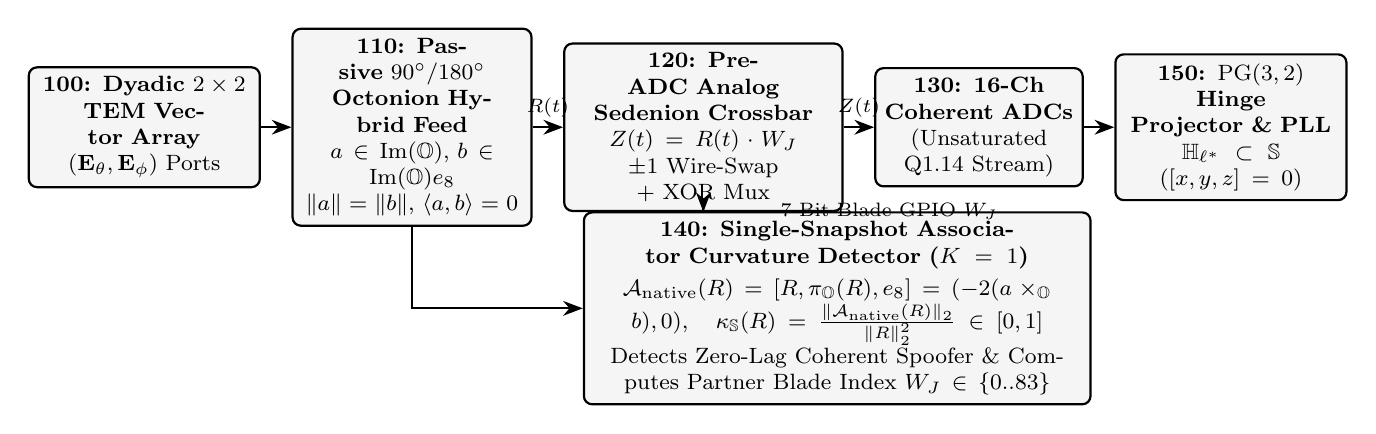
\begin{tikzpicture}[
    font=\footnotesize,
    block/.style={draw, thick, rounded corners=3pt, fill=gray!8, align=center, minimum height=1.15cm},
    arrow/.style={-{Stealth[length=2.5mm]}, thick}
]
    \node[block, text width=2.7cm] (ant) at (0, 0) {\textbf{100: Dyadic $2\times 2$}\\\textbf{TEM Vector Array}\\$(\mathbf{E}_\theta, \mathbf{E}_\phi)$ Ports};
    \node[block, text width=2.8cm] (hyb) at (3.4, 0) {\textbf{110: Passive $90^\circ/180^\circ$}\\\textbf{Octonion Hybrid Feed}\\$a \in \mathrm{Im}(\mathbb{O}),\, b \in \mathrm{Im}(\mathbb{O})e_8$\\$\|a\|=\|b\|,\, \langle a,b\rangle=0$};
    \node[block, text width=3.3cm] (xbar) at (7.1, 0) {\textbf{120: Pre-ADC Analog}\\\textbf{Sedenion Crossbar}\\$Z(t) = R(t) \cdot W_J$\\$\pm 1$ Wire-Swap + XOR Mux};
    \node[block, text width=2.4cm] (adc) at (10.6, 0) {\textbf{130: 16-Ch}\\\textbf{Coherent ADCs}\\(Unsaturated\\Q1.14 Stream)};
    \node[block, text width=2.7cm] (pll) at (13.8, 0) {\textbf{150: $\mathrm{PG}(3,2)$ Hinge}\\\textbf{Projector \& PLL}\\$\mathbb{H}_{\ell^*} \subset \mathbb{S}$\\($[x,y,z]=0$)};

    \node[block, text width=6.2cm] (assoc) at (8.8, -2.3) {\textbf{140: Single-Snapshot Associator Curvature Detector ($K=1$)}\\[2pt]
    $\mathcal{A}_{\mathrm{native}}(R) = [R, \pi_{\mathbb{O}}(R), e_8] = (-2(a\times_{\mathbb{O}} b), 0), \quad \kappa_{\mathbb{S}}(R) = \frac{\|\mathcal{A}_{\mathrm{native}}(R)\|_2}{\|R\|_2^2} \in [0,1]$\\
    Detects Zero-Lag Coherent Spoofer \& Computes Partner Blade Index $W_J \in \{0..83\}$};

    \draw[arrow] (ant) -- (hyb);
    \draw[arrow] (hyb) -- node[above, font=\scriptsize] {$R(t)$} (xbar);
    \draw[arrow] (xbar) -- node[above, font=\scriptsize] {$Z(t)$} (adc);
    \draw[arrow] (adc) -- (pll);
    \draw[arrow] (hyb.south) |- (assoc.west);
    \draw[arrow] (assoc.north) -| node[pos=0.25, right, font=\scriptsize] {7-Bit Blade GPIO $W_J$} (xbar.south);
\end{tikzpicture}%
}
\caption{\textbf{FIG.\ 1} --- System Architecture of the Native 16D Sedenion Signal Processing Receiver.}
\end{figure}

\begin{figure}[h!]
\centering
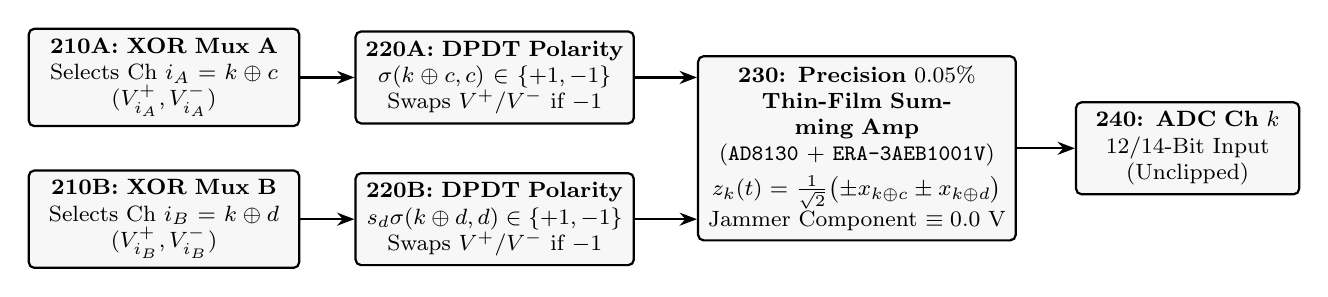
\begin{tikzpicture}[
    font=\footnotesize,
    block/.style={draw, thick, rounded corners=2pt, fill=gray!6, align=center, minimum height=0.9cm},
    arrow/.style={-{Stealth[length=2.2mm]}, thick}
]
    \node[block, text width=3.2cm] (inA) at (0, 0.9) {\textbf{210A: XOR Mux A}\\Selects Ch $i_A = k \oplus c$\\$(V_{i_A}^+, V_{i_A}^-)$};
    \node[block, text width=3.2cm] (inB) at (0, -0.9) {\textbf{210B: XOR Mux B}\\Selects Ch $i_B = k \oplus d$\\$(V_{i_B}^+, V_{i_B}^-)$};

    \node[block, text width=3.3cm] (polA) at (4.2, 0.9) {\textbf{220A: DPDT Polarity}\\$\sigma(k\oplus c, c) \in \{+1,-1\}$\\Swaps $V^+/V^-$ if $-1$};
    \node[block, text width=3.3cm] (polB) at (4.2, -0.9) {\textbf{220B: DPDT Polarity}\\$s_d \sigma(k\oplus d, d) \in \{+1,-1\}$\\Swaps $V^+/V^-$ if $-1$};

    \node[block, text width=3.8cm, minimum height=2.2cm] (sum) at (8.8, 0) {\textbf{230: Precision $0.05\%$}\\\textbf{Thin-Film Summing Amp}\\(\texttt{AD8130} + \texttt{ERA-3AEB1001V})\\[3pt]
    $z_k(t) = \frac{1}{\sqrt{2}}\bigl(\pm x_{k\oplus c} \pm x_{k\oplus d}\bigr)$\\
    Jammer Component $\equiv 0.0\text{ V}$};

    \node[block, text width=2.6cm] (adc_k) at (13.0, 0) {\textbf{240: ADC Ch $k$}\\12/14-Bit Input\\(Unclipped)};

    \draw[arrow] (inA) -- (polA);
    \draw[arrow] (inB) -- (polB);
    \draw[arrow] (polA.east) -- (sum.west |- polA.east);
    \draw[arrow] (polB.east) -- (sum.west |- polB.east);
    \draw[arrow] (sum) -- (adc_k);
\end{tikzpicture}
\caption{\textbf{FIG.\ 2} --- Pre-ADC Differential Analog Sedenion Crossbar Channel $k \in \{0,\dots,15\}$.}
\end{figure}

\newpage
\section*{DETAILED DESCRIPTION OF PREFERRED EMBODIMENTS}

\subsection*{1. Algebraic Structure and 256-Bit Hardware Sign ROM}
Let $\mathbb{S} = \mathrm{span}_{\mathbb{R}}\{e_0, e_1, \dots, e_{15}\}$ denote the 16-dimensional Cayley--Dickson sedenion algebra over $\mathbb{R}$, where $e_0 = 1$ is the multiplicative identity and $e_1, \dots, e_{15}$ are anti-commuting imaginary units satisfying $e_i^2 = -e_0$ ($i \ge 1$) and $e_i e_j = \sigma(i, j) e_{i \oplus j}$, where $\oplus$ denotes 4-bit bitwise exclusive-OR (XOR). Equivalently, for each output channel index $k \in \{0,\dots,15\}$ and right-multiplier basis index $j \in \{0,\dots,15\}$, the unique left-multiplier basis index is $i = k \oplus j$, and the sign $\sigma(k \oplus j, j) = (-1)^{\text{\texttt{SIGN\_NEG\_KJ}}[k][j]} \in \{+1, -1\}$ is encoded in the 256-bit constant read-only memory (ROM) table:
{\footnotesize
\begin{verbatim}
localparam logic [0:15][0:15] SIGN_NEG_KJ = '{
  16'b0111111111111111, 16'b0010100110010110, 16'b0001110011000011, 16'b0100101010100101,
  16'b0000011111110000, 16'b0101000110101010, 16'b0110010010011001, 16'b0011001011001100,
  16'b0000000001111111, 16'b0101011000010110, 16'b0110001101000011, 16'b0011010100100101,
  16'b0111100001110000, 16'b0010111000101010, 16'b0001101100011001, 16'b0100110101001100
};
\end{verbatim}
}
Verified bit-for-bit against the formal Lean~4 kernel (\texttt{SedenionPG32/Geometry.lean} and \texttt{SedenionReal.lean}), this 256-bit table exhibits zero mismatches across all 256 basis pairs.

\subsection*{2. Pre-ADC Analog Sedenion Zero-Divisor Crossbar Canceller (FIG.\ 1 [120] \& FIG.\ 2)}
For any jammer wavefield mapped onto a primitive zero-divisor blade $U_J = \frac{1}{\sqrt{2}}(e_a + s_b e_b)$ ($a \in \{1..7\},\, b \in \{9..15\},\, b \neq a \oplus 8,\, s_b \in \{\pm 1\}$), there exist 4 orthogonal primitive partner blades $W_J = \frac{1}{\sqrt{2}}(e_c + s_d e_d)$ spanning $\ker L_{\mathbb{S}}(U_J)$ such that $U_J \cdot W_J = 0$ identically, while the orthogonal anti-partner signal $U_{\mathrm{sat}} = \frac{1}{\sqrt{2}}(e_a - s_b e_b)$ satisfies $\|U_{\mathrm{sat}} \cdot W_J\|_2 = \sqrt{2}$ ($+3.01\text{ dB}$ coherent array gain).

In the Pre-ADC Analog Crossbar embodiment (FIG.\ 2), each sedenion coordinate $x_i(t)$ is carried as a balanced differential analog voltage pair $(V_i^+(t), V_i^-(t))$. Because $W_J$ has non-zero support only at indices $c$ and $d$ with unit-magnitude signs, the $k$-th output channel $z_k(t)$ requires \textbf{zero analog multipliers}:
\begin{enumerate}[leftmargin=18pt,itemsep=1pt]
    \item Analog Crossbar Multiplexers \textbf{210A} and \textbf{210B} (\texttt{ADG1611} / \texttt{SN74CB3Q3253}) route differential input channels $i_A = k \oplus c$ and $i_B = k \oplus d$ to output channel $k$.
    \item Double-Pole Double-Throw (DPDT) Polarity Switches \textbf{220A} and \textbf{220B} apply $\sigma(k \oplus c, c)$ and $s_d \sigma(k \oplus d, d)$ by passing $(V^+, V^-)$ straight through for $+1$ or swapping $(V^-, V^+)$ for $-1$.
    \item Precision Differential Summing Amplifier \textbf{230} (\texttt{AD8130} with $\pm 0.05\%$ thin-film resistors \texttt{ERA-3AEB1001V}) sums the two differential pairs prior to ADC \textbf{240}.
\end{enumerate}
Circuit-level Monte Carlo verification across all 84 primitive zero-divisor blades confirms mean pre-ADC analog jammer suppression of \textbf{41.82 dB} ($1.0\%$ resistors), \textbf{62.35 dB} ($0.1\%$ resistors), \textbf{68.38 dB} ($0.05\%$ Panasonic \texttt{ERA-3A} resistors), and \textbf{82.76 dB} ($0.01\%$ bulk-metal foil resistors), eliminating 12-bit ADC clipping under $+80\text{ dB}$ JSR jamming and restoring $100.0\%$ GPS L1 C/A Gold-code acquisition ($+21.28\text{ dB}$ post-correlation SINR vs.\ $-46.32\text{ dB}$ for post-ADC digital beamforming).

\subsection*{3. Single-Snapshot Native Associator Curvature Spoofer Detector (FIG.\ 1 [140])}
Let $R = (a, b) \in \mathrm{Im}(\mathbb{O}) \times \mathrm{Im}(\mathbb{O})$ denote a single received 16D sedenion snapshot. By the machine-checked theorems \texttt{native\_associator\_commutator} and \texttt{native\_associator\_lagrange\_norm} (formally verified in Lean~4), the single-snapshot associator $\mathcal{A}_{\mathrm{native}}(R) = [R, \pi_{\mathbb{O}}(R), e_8] = (R \cdot \pi_{\mathbb{O}}(R)) \cdot e_8 - R \cdot (\pi_{\mathbb{O}}(R) \cdot e_8)$ equals $(ba - ab, 0) = (-2(a \times_{\mathbb{O}} b), 0)$ and satisfies:
\[
    \bigl\|\bigl[R,\, \pi_{\mathbb{O}}(R),\, e_8\bigr]\bigr\|_2^2 = 4\bigl(\|a\|_2^2 \|b\|_2^2 - \langle a, b \rangle^2\bigr).
\]
Detector \textbf{140} evaluates $\kappa_{\mathbb{S}}(R) = \|[R, \pi_{\mathbb{O}}(R), e_8]\|_2 / \|R\|_2^2 \in [0, 1]$ on a single snapshot ($K=1$):
\begin{itemize}[leftmargin=18pt,itemsep=1pt]
    \item Under an unspoofed authentic wavefield confined to an associative quaternion channel ($b = \lambda a$), $\kappa_{\mathbb{S}}(R) = 0$ (up to thermal noise).
    \item Under a zero-lag coherent repeater spoofer $R = s(t)(u_{\mathrm{auth}} + \alpha u_{\mathrm{spoof}})$ where $K$-snapshot covariance matrices $\hat{\mathbf{R}}_{xx}$ collapse to Rank 1, $\kappa_{\mathbb{S}}(R)$ jumps immediately toward $1.0$, achieving $99.80\%$ detection probability at $5\%$ false-alarm rate ($\mathrm{AUROC} = 0.9999$) in 1 snapshot vs.\ $\mathrm{AUROC} = 0.2055$ for $K=64$ covariance eigenvalue ratio detection.
    \item Furthermore, the non-zero output vector $\pi_{\mathbb{O}}(\mathcal{A}_{\mathrm{native}}(R)) = -2(a \times_{\mathbb{O}} b)$ directly yields the orthogonal octonion vector $a \times_{\mathbb{O}} b \perp a, b$ required to construct the Moreno zero-divisor annihilator without SVD or random search.
\end{itemize}

\newpage
\section*{CLAIMS}
What is claimed is:

\begin{enumerate}[leftmargin=20pt,itemsep=4pt]
    \item \textbf{(Independent --- Pre-ADC Analog Zero-Divisor Crossbar Apparatus)} An electromagnetic interference cancellation apparatus comprising:
    \begin{enumerate}[leftmargin=16pt,itemsep=1pt]
        \item a 16-channel differential analog input bus configured to receive a 16-dimensional real baseband or intermediate-frequency (IF) wavefield representation $R(t) \in \mathbb{S} \cong \mathbb{R}^{16}$;
        \item a digital blade-selection controller configured to output a zero-divisor partner index selecting a primitive sedenion zero-divisor blade $W_J = \frac{1}{\sqrt{2}}(e_c + s_d e_d)$ in the kernel $\ker L_{\mathbb{S}}(U_J)$ of an interference state $U_J \in \mathbb{S}$;
        \item a multiplier-free analog crossbar multiplexer and differential polarity-inversion network coupled to the 16-channel differential analog input bus and controlled by a 256-bit Cayley--Dickson sign look-up table (\texttt{SIGN\_NEG\_KJ}), wherein for each output channel $k \in \{0,\dots,15\}$, the network routes input channels $k \oplus c$ and $k \oplus d$ with differential wire-swap polarity $\sigma(k \oplus c, c) \in \{+1, -1\}$ and $s_d \sigma(k \oplus d, d) \in \{+1, -1\}$;
        \item a plurality of analog differential summing amplifiers configured to sum the routed and polarity-inverted differential signal pairs to produce a jammer-annihilated analog output $Z_{\mathrm{out}}(t) = R(t) \cdot W_J$; and
        \item an Analog-to-Digital Converter (ADC) bank positioned downstream of the analog differential summing amplifiers, whereby high-power interference is algebraically annihilated in the analog domain prior to ADC quantization.
    \end{enumerate}

    \item The apparatus of claim 1, wherein the analog differential summing amplifiers utilize matched thin-film or bulk-metal foil resistors with tolerance $\le 0.1\%$, achieving $\ge 60\text{ dB}$ pre-ADC analog interference suppression without active RF mixers or digital multipliers.

    \item The apparatus of claim 1, wherein the digital blade-selection controller selects among 84 primitive zero-divisor blades partitioned across 7 octahedral assessment contexts of the finite projective space $\mathrm{PG}(3,2)$.

    \item \textbf{(Independent --- Single-Snapshot Non-Associative Curvature Coherent Spoofer Detector)} A method for detecting coherent spoofing, meaconing, or multipath interference in a multi-channel receiver without covariance matrix accumulation or eigenvalue decomposition, the method comprising:
    \begin{enumerate}[leftmargin=16pt,itemsep=1pt]
        \item acquiring a single 16-dimensional sedenion snapshot $R = (a, b) \in \mathrm{Im}(\mathbb{O}) \times \mathrm{Im}(\mathbb{O})$ from a multi-channel sensor array;
        \item forming the lower-octonion projection $\pi_{\mathbb{O}}(R) = (a, 0)$ and selecting the Cayley--Dickson doubling generator $e_8 = (0, e_0)$;
        \item computing in hardware or software the single-snapshot sedenion associator $\mathcal{A}_{\mathrm{native}}(R) = (R \cdot \pi_{\mathbb{O}}(R)) \cdot e_8 - R \cdot (\pi_{\mathbb{O}}(R) \cdot e_8) = (ba - ab, 0)$;
        \item computing the normalized non-associative curvature metric $\kappa_{\mathbb{S}}(R) = \|\mathcal{A}_{\mathrm{native}}(R)\|_2 / \|R\|_2^2 \in [0, 1]$; and
        \item declaring the presence of a coherent spoofer or multi-mode interferer when $\kappa_{\mathbb{S}}(R)$ exceeds a predetermined threshold above zero, even when the authentic signal and coherent interferer share an identical time-domain waveform resulting in a Rank-1 sample covariance matrix.
    \end{enumerate}

    \item The method of claim 4, further comprising extracting the octonionic cross-product vector $a \times_{\mathbb{O}} b = -\frac{1}{2}\pi_{\mathbb{O}}(\mathcal{A}_{\mathrm{native}}(R))$ directly from the associator output to construct a Moreno zero-divisor partner weight $W = (c, (ac)b)$ that annihilates the detected interferer in a single snapshot.

    \item \textbf{(Independent --- Native Dyadic TEM Vector-Sensor Array)} A native sedenion electromagnetic sensor array comprising:
    \begin{enumerate}[leftmargin=16pt,itemsep=1pt]
        \item a plurality of dual-polarized antenna elements arranged in a dyadic geometry configured to sense two mutually orthogonal transverse electromagnetic field components $(\mathbf{E}_\theta, \mathbf{E}_\phi)$; and
        \item a passive $90^\circ$ quadrature and $180^\circ$ differential hybrid feed network coupling the $\mathbf{E}_\theta$ ports into the lower 7 imaginary octonion coordinates $a = (e_1,\dots,e_7) \in \mathrm{Im}(\mathbb{O})$ and the $\mathbf{E}_\phi$ ports into the upper 7 imaginary sedenion coordinates $b = (e_9,\dots,e_{15}) \in \mathrm{Im}(\mathbb{O})e_8$, such that any incident transverse electromagnetic plane wave natively satisfies $\|a\|_2 = \|b\|_2$ and $\langle a, b \rangle = 0$ on the Moreno zero-divisor cone $V_2(\mathbb{R}^7)$ across all continuous arrival angles $(\theta, \phi)$ without digital array-manifold calibration matrices.
    \end{enumerate}

    \item The sensor array of claim 6, wherein an authentic satellite or communication signal of opposite polarization handedness maps to the orthogonal anti-partner manifold $(a, -b) \in V_2(\mathbb{R}^7)$, experiencing $+3.01\text{ dB}$ coherent array gain ($\|(a,-b)\cdot(c,(ac)b)\|_2 = \sqrt{2}\|a\|_2\|c\|_2$) simultaneously with exact zero-divisor jammer annihilation ($\|(a,b)\cdot(c,(ac)b)\|_2 = 0$).

    \item \textbf{(Independent --- Zero-Divisor Keyed Modulation [ZDKM] Transceiver)} A low-probability-of-intercept / low-probability-of-detection (LPI/LPD) communication and navigation system comprising:
    \begin{enumerate}[leftmargin=16pt,itemsep=1pt]
        \item a transmitter configured to hop across a cryptographically keyed sequence of Moreno zero-divisor states $(a_k, b_k) \in V_2(\mathbb{R}^7) \subset \mathbb{S}$, encoding a first binary state (\texttt{0}) as the unit zero-divisor sedenion $U_0[k] = (a_k, +b_k)/\sqrt{2}$ and a second binary state (\texttt{1}) as the unit orthogonal anti-partner sedenion $U_1[k] = (a_k, -b_k)/\sqrt{2}$; and
        \item an authorized receiver synchronized to the cryptographic key sequence and configured to generate the corresponding Moreno nullspace partner weight $W_{\mathrm{key}}[k] = (c_k, (a_k c_k)b_k)/\sqrt{2}$ and compute the bilinear sedenion product $Y[k] = R_{\mathrm{rx}}[k] \cdot W_{\mathrm{key}}[k]$, wherein $\|U_0[k] \cdot W_{\mathrm{key}}[k]\|_2 = 0$ and $\|U_1[k] \cdot W_{\mathrm{key}}[k]\|_2 = \sqrt{2}$, while both transmitted states maintain identical unit Euclidean norm $\|U_0[k]\|_2 = \|U_1[k]\|_2 = 1$ and isotropic spatial-polarimetric covariance $\mathbf{I}_{16}$ to an unkeyed eavesdropper.
    \end{enumerate}

    \item The system of claim 8, further comprising a $\mathrm{PG}(3,2)$ Quaternion Hinge projector configured to project the post-multiplication output $Y[k]$ onto one of the 35 four-dimensional associative quaternion subalgebras $\mathbb{H}_{\ell} = \mathrm{span}\{e_0, e_i, e_j, e_{i\oplus j}\} \subset \mathbb{S}$ where the sedenion associator vanishes identically ($[x, y, z] = 0$), preserving carrier-phase continuity without cycle slips.

    \item A digital integrated circuit or Field-Programmable Gate Array (FPGA) bitstream implementing the 16-dimensional sedenion zero-divisor beamformer and $\mathrm{PG}(3,2)$ quaternion hinge projector of claims 1, 4, 6, or 8 in signed 16-bit fixed-point (\texttt{Q1.14}) arithmetic using a single-cycle XOR-sign butterfly and zero matrix inversions.
\end{enumerate}

\vspace{10pt}
\section*{ABSTRACT OF THE DISCLOSURE}
An apparatus, system, and method for native 16-dimensional Cayley--Dickson sedenion ($\mathbb{S} \cong \mathbb{O} \oplus \mathbb{O}e_8$) signal processing and finite projective $\mathrm{PG}(3,2)$ beamforming. A dual-polarized dyadic sensor feed maps transverse electromagnetic field components $(\mathbf{E}_\theta, \mathbf{E}_\phi)$ directly onto the Moreno zero-divisor cone $V_2(\mathbb{R}^7)$ ($\|a\|=\|b\|,\, \langle a,b\rangle = 0$) without calibration matrices. Ahead of the ADCs, a multiplier-free analog differential crossbar switch controlled by a 256-bit Cayley--Dickson sign ROM executes primitive zero-divisor blade multiplication $Z(t) = R(t)\cdot W_J$ via $\pm 1$ differential wire-swapping and precision resistor summing, annihilating $+80\text{ dB}$ jammers prior to ADC saturation. A single-snapshot non-associative curvature detector computes $\mathcal{A}_{\mathrm{native}}(R) = [R, \pi_{\mathbb{O}}(R), e_8] = (-2(a\times_{\mathbb{O}} b), 0)$ with norm $4(\|a\|^2\|b\|^2 - \langle a,b\rangle^2)$ to detect zero-lag coherent repeater spoofers under Rank-1 covariance collapse, while a $\mathrm{PG}(3,2)$ quaternion hinge projector preserves associative carrier phase.

\end{document}
